% Coco, second presentation (status update 2)
% build: cd docs/slides/presentation_2 && pdflatex coco.tex && pdflatex coco.tex
%   -> coco.pdf (public, in git): The Office characters as name badges
% with faces (for the talk, local only): ./build-faces.sh -> coco-faces.pdf
%   faces go in faces/michael.jpg, jim.jpg, pam.jpg, toby.jpg, angela.jpg (git-ignored: actors' photos,
%   fine in class, but not for the public repo)
% same look as presentation_1 (black and white, grey cards, bar left of the titles, panda)
\documentclass[aspectratio=169,11pt]{beamer}

\usepackage[T1]{fontenc}
\usepackage{lmodern}
\usepackage{tikz}
\usetikzlibrary{positioning,calc,arrows.meta}

% >>> set the date of the talk here <<<
\newcommand{\talkdate}{27 November 2026}

% images live in the app, app-pictures and presentation_1 folders, no copies
\graphicspath{{../../../ios/Coco/Assets.xcassets/panda-idle.imageset/}
              {../../../ios/Coco/Assets.xcassets/panda-listening.imageset/}
              {../../../ios/Coco/Assets.xcassets/panda-thinking.imageset/}
              {../../../ios/Coco/Assets.xcassets/panda-talking.imageset/}
              {../../app-pictures/}
              {../presentation_1/}}

% black and white + the app's soft grey cards
\definecolor{card}{gray}{0.945}
\definecolor{soft}{gray}{0.42}
\definecolor{accent}{gray}{0.45} % highlight cards

\setbeamersize{text margin left=1cm,text margin right=1cm}
\setbeamertemplate{navigation symbols}{}
\setbeamercolor{normal text}{fg=black,bg=white}
\setbeamercolor{frametitle}{fg=black,bg=white}
\setbeamercolor{title}{fg=black}
\setbeamercolor{structure}{fg=black}
\setbeamerfont{frametitle}{series=\bfseries,size=\Large}
\setbeamertemplate{itemize items}{\textbullet}

% title with a thick bar on its left
\setbeamertemplate{frametitle}{%
  \vskip0.5cm{\usebeamerfont{frametitle}\rule[-0.22em]{3.5pt}{1.15em}\hspace{0.28cm}\insertframetitle\par}%
  \vskip0.3cm}

% page number bottom right
\setbeamertemplate{footline}{%
  \hfill\raisebox{0.1cm}{\textcolor{soft}{\scriptsize\insertframenumber}}\hspace{0.45cm}\vspace{0.2cm}}

% no word breaks anywhere
\AtBeginDocument{\hyphenpenalty=10000\exhyphenpenalty=10000}

\tikzset{
  card/.style={fill=card,rounded corners=6pt,inner sep=7pt,align=left,anchor=north west},
  chip/.style={fill=card,rounded corners=4pt,align=center,font=\scriptsize,
               text width=1.32cm,minimum height=0.95cm,inner sep=2pt},
  dark/.style={fill=accent,text=white},
}

% card content that starts at the top, so cards in a row line up
\newcommand{\topbox}[3]{\parbox[t][#2][t]{#1}{\raggedright #3}}
% bullet whose wrapped lines stay indented
\newcommand{\bul}[1]{\par\hangindent=0.85em\hangafter=1\noindent\textbullet\ #1\par\vspace{3pt}}
% agent card: name + one small line
\newcommand{\agent}[2]{\textbf{#1}\\[-1pt]{\scriptsize #2}}
% phone screenshot, rounded corners + thin grey frame: \phone{x}{y}{height}{file}
% (shows the top part of the screenshot; width = 0.578 x height, like an iPhone screen)
\newcommand{\phone}[4]{%
  \pgfmathsetmacro{\phw}{0.578*#3}%
  \begin{scope}
    \clip[rounded corners=7pt] (#1,#2) rectangle ++(\phw,-#3);
    \node[anchor=north west,inner sep=0pt] at (#1,#2) {\includegraphics[width=\phw cm]{#4}};
  \end{scope}
  \draw[soft!60,rounded corners=7pt,line width=0.5pt] (#1,#2) rectangle ++(\phw,-#3);}
% a The Office character on the test chart: face (only in the local faces build) or a name badge
% \officeface{x}{y}{file name}{initial}
\newcommand{\officeface}[4]{%
  \ifdefined\withfaces
    \IfFileExists{faces/#3.jpg}{%
      \node[circle,draw=soft,thick,inner sep=0pt,minimum size=0.52cm,
            path picture={\node at (path picture bounding box.center)
              {\includegraphics[height=0.56cm]{faces/#3.jpg}};}] at (#1,#2) {};}%
      {\node[circle,draw=soft,thick,fill=white,inner sep=0pt,minimum size=0.44cm,font=\tiny\bfseries] at (#1,#2) {#4};}%
  \else
    \node[circle,draw=soft,thick,fill=white,inner sep=0pt,minimum size=0.44cm,font=\tiny\bfseries] at (#1,#2) {#4};
  \fi}
% small grey line under a slide
\newcommand{\smallnote}[1]{{\scriptsize\textcolor{soft}{#1}}}

\begin{document}

% ───────────────────────── 1. title ─────────────────────────
\begin{frame}[plain]
  \begin{columns}[c]
    \begin{column}{0.56\textwidth}
      {\fontsize{54}{58}\selectfont\bfseries Coco}\\[0.5em]
      {\large A digital everyday-assistance service for older adults, staffed by AI agents}\\[0.9em]
      \rule{1.3cm}{2pt}\\[0.7em]
      {\small Status update 2\\ Ren, Xingyu\\ \textcolor{soft}{Frontier Systems 2026/27 \,$\cdot$\, \talkdate}}
    \end{column}
    \begin{column}{0.38\textwidth}
      \centering
      
\includegraphics[width=\textwidth]{panda-idle}
    \end{column}
  \end{columns}
\end{frame}


% ───────────────────────── 2. where we were ─────────────────────────
\begin{frame}[t]{Where we were, and what's new}
  \vspace*{0.1cm}
  {\small Coco: an AI helper app for \textbf{older adults living alone}, paid by their children, for \textbf{Germany and China}.}\par\vspace{0.7em}
  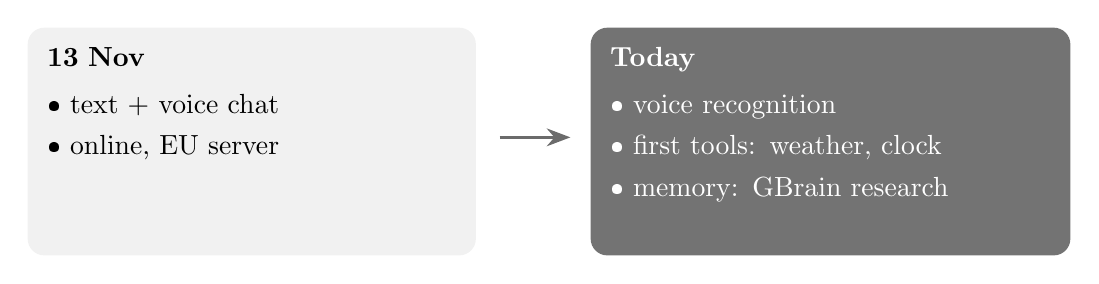
\begin{tikzpicture}
    \node[card,text width=5.2cm] at (0,0) {\topbox{5.2cm}{2.4cm}{%
      \textbf{13 Nov}\par\vspace{0.5em}
      \bul{text + voice chat}
      \bul{online, EU server}}};
    \draw[-{Stealth[length=3mm]},very thick,soft] (6.0,-1.4) -- (6.9,-1.4);
    \node[card,dark,text width=5.6cm] at (7.15,0) {\topbox{5.6cm}{2.4cm}{%
      \textbf{Today}\par\vspace{0.5em}
      \bul{voice recognition}
      \bul{first tools: weather, clock}
      \bul{memory: GBrain research}}};
  \end{tikzpicture}
\end{frame}

% ───────────────────────── 3. language ─────────────────────────
\begin{frame}[t]{English demo now, Chinese models for real users}
  \vspace*{-0.1cm}
  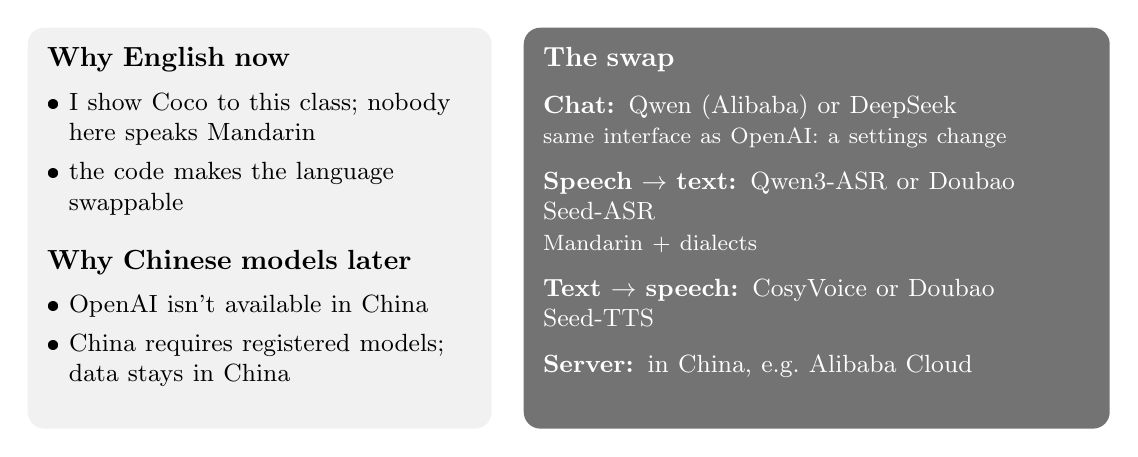
\begin{tikzpicture}
    \node[card,text width=5.4cm] at (0,0) {\topbox{5.4cm}{4.6cm}{%
      \textbf{Why English now}\par\vspace{0.5em}\small
      \bul{I show Coco to this class; nobody here speaks Mandarin}
      \bul{the code makes the language swappable}\par\vspace{0.8em}
      \textbf{\normalsize Why Chinese models later}\par\vspace{0.5em}
      \bul{OpenAI isn't available in China}
      \bul{China requires registered models; data stays in China}}};
    \node[card,dark,text width=6.95cm] at (6.3,0) {\topbox{6.95cm}{4.6cm}{%
      \textbf{The swap}\par\vspace{0.6em}\small
      \textbf{Chat:} Qwen (Alibaba) or DeepSeek\par
      {\footnotesize same interface as OpenAI: a settings change}\par\vspace{0.6em}
      \textbf{Speech $\to$ text:} Qwen3-ASR or Doubao Seed-ASR\par
      {\footnotesize Mandarin + dialects}\par\vspace{0.6em}
      \textbf{Text $\to$ speech:} CosyVoice or Doubao Seed-TTS\par\vspace{0.6em}
      \textbf{Server:} in China, e.g.\ Alibaba Cloud}};
  \end{tikzpicture}
\end{frame}

% ───────────────────────── 4. voiceprint ─────────────────────────
\begin{frame}[t]{Voice recognition: is this the user talking?}
  \vspace*{-0.2cm}
  \begin{tikzpicture}
    \phone{0}{0}{5.4}{voiceprint-you}
    \phone{3.3}{0}{5.4}{voiceprint-someone-else}
    \node[font=\scriptsize,text=soft] at (1.56,-5.65) {me $\to$ 0.70};
    \node[font=\scriptsize,text=soft] at (4.86,-5.65) {Pam (TV) $\to$ 0.20};
    \begin{scope}[every node/.style={card,text width=6.2cm,inner sep=6pt,font=\small}]
      \node (a) at (7.0,0) {\textbf{How}\par\footnotesize
        voice $\to$ 192 numbers (a ``fingerprint''), compared with the user's. Open source: SpeechBrain.};
      \node[below=0.15cm of a.south west,anchor=north west] (b) {\textbf{Safe}\par\footnotesize
        runs on our own server; we keep only the numbers, never the audio; deletable.};
      \node[dark,below=0.15cm of b.south west,anchor=north west] {\textbf{What Coco does with it}\par\footnotesize
        visitors get no private info $\cdot$ notices the TV $\cdot$ emergencies count from anyone $\cdot$ later: memory only saves the user's words};
    \end{scope}
  \end{tikzpicture}
\end{frame}

% ───────────────────────── 5. voiceprint: test ─────────────────────────
\begin{frame}[t]{How we tested it: me, a friend, and \emph{The Office}}
  \vspace*{-0.25cm}
  {\small Set up once with my voice, then tried: me, a friend, and \emph{The Office} on TV.}\par\vspace{0.3em}
  \centering
  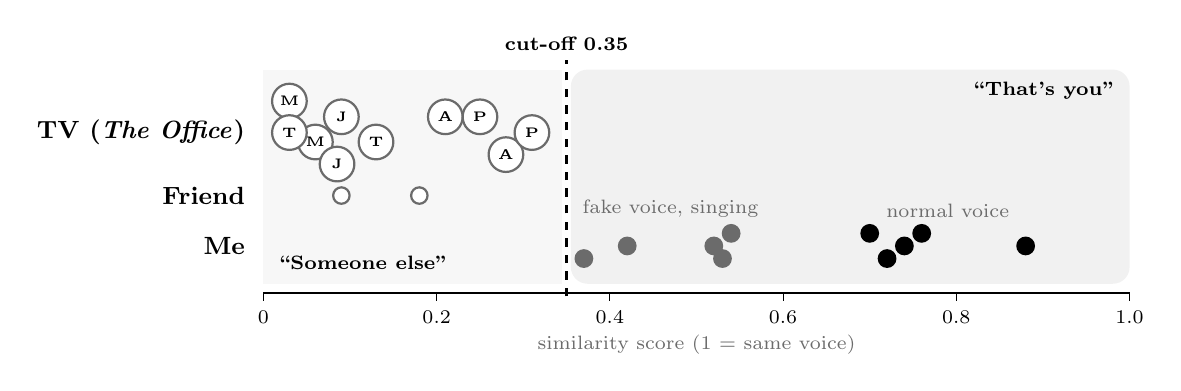
\begin{tikzpicture}[x=11.0cm,y=0.8cm,
      other/.style={circle,draw=soft,fill=white,thick,inner sep=2.1pt},
      me/.style={circle,fill=black,inner sep=2.4pt},
      odd/.style={circle,fill=soft,inner sep=2.4pt},
      lab/.style={font=\scriptsize,text=soft}]
    % zones
    \fill[card!55!white] (0,0.15) rectangle (0.345,3.55);
    \fill[card] (0.355,0.15) rectangle (1,3.55);
    \node[font=\scriptsize\bfseries,anchor=south west] at (0.005,0.22) {``Someone else''};
    \node[font=\scriptsize\bfseries,anchor=north east] at (0.995,3.5) {``That's you''};
    % axis
    \draw[thick] (0,0) -- (1,0);
    \foreach \t in {0,0.2,0.4,0.6,0.8,1.0}{ \draw (\t,0) -- (\t,-0.12) node[below,font=\scriptsize] {\t}; }
    \node[lab,anchor=north] at (0.5,-0.5) {similarity score (1 = same voice)};
    % cut-off
    \draw[dashed,thick] (0.35,-0.05) -- (0.35,3.7);
    \node[font=\scriptsize\bfseries,anchor=south] at (0.35,3.7) {cut-off 0.35};
    % rows
    \node[font=\small\bfseries,anchor=east] at (-0.01,2.55) {TV (\emph{The Office})};
    \node[font=\small\bfseries,anchor=east] at (-0.01,1.55) {Friend};
    \node[font=\small\bfseries,anchor=east] at (-0.01,0.75) {Me};
    % The Office: two tries each (Mac, online); y nudged so faces don't overlap
    \officeface{0.03}{3.05}{michael}{M}  \officeface{0.06}{2.4}{michael}{M}
    \officeface{0.09}{2.8}{jim}{J}       \officeface{0.085}{2.05}{jim}{J}
    \officeface{0.03}{2.55}{toby}{T}     \officeface{0.13}{2.4}{toby}{T}
    \officeface{0.21}{2.8}{angela}{A}    \officeface{0.28}{2.2}{angela}{A}
    \officeface{0.25}{2.8}{pam}{P}       \officeface{0.31}{2.55}{pam}{P}
    \foreach \v in {0.09,0.18}{ \node[other] at (\v,1.55) {}; }
    % me: normal voice (black), fake voice + singing (grey)
    \foreach \v/\y in {0.74/0.75,0.76/0.95,0.88/0.75,0.70/0.95,0.72/0.55}{ \node[me] at (\v,\y) {}; }
    \foreach \v/\y in {0.42/0.75,0.53/0.55,0.54/0.95,0.52/0.75,0.37/0.55}{ \node[odd] at (\v,\y) {}; }
    \node[lab,anchor=south] at (0.79,1.05) {normal voice};
    \node[lab,anchor=south] at (0.47,1.05) {fake voice, singing};
  \end{tikzpicture}\\[0.25em]
  \raggedright
  \ifdefined\withfaces
    \smallnote{27 tries on the Mac and the online server, all sorted correctly. Closest: Pam 0.31 vs.\ my singing 0.37.}\par
    {\fontsize{5}{6}\selectfont\textcolor{soft}{Photos from the Office years via Wikimedia Commons, cropped: Steve Carell (2007) by StacyD (CC BY 3.0);
    John Krasinski, Jenna Fischer, Angela Kinsey (2009) by Kristin Dos Santos (CC BY-SA 2.0); Paul Lieberstein (2008) by NoHoDamon (CC BY-SA 2.0).}}
  \else
    \smallnote{M Michael, J Jim, P Pam, T Toby, A Angela. 27 tries on the Mac and the online server, all sorted correctly.
    Closest: Pam 0.31 vs.\ my singing 0.37. Small test: keep testing.}
  \fi
\end{frame}


% ───────────────────────── 6. tools ─────────────────────────
\begin{frame}[t]{First tools: weather and clock}
  \vspace*{-0.2cm}
  \begin{tikzpicture}[
      st/.style={card,text width=5.95cm,inner sep=5pt,font=\small},
      arr/.style={-{Stealth[length=2mm]},semithick,soft}]
    \phone{0}{0}{5.6}{weather-card}
    \phone{3.45}{0}{5.6}{clock}
    \node[font=\small\bfseries,anchor=south west,inner sep=0pt] at (7.1,0.1) {How a tool works};
    \node[st] (s1) at (7.1,-0.2) {\textbf{1.} you ask: ``Is it cold outside?''};
    \node[st,below=0.32cm of s1.south west,anchor=north west] (s2) {\textbf{2.} the LLM picks a tool: get\_weather(Hannover)};
    \node[st,dark,below=0.32cm of s2.south west,anchor=north west] (s3) {\textbf{3.} our server runs it (Open-Meteo)};
    \node[st,below=0.32cm of s3.south west,anchor=north west] (s4) {\textbf{4.} the LLM answers, the app shows a card};
    \foreach \a/\b in {s1/s2,s2/s3,s3/s4}{ \draw[arr] (\a.south) -- (\b.north); }
    \node[anchor=north west,text width=5.95cm,font=\footnotesize,inner sep=0pt] at ([yshift=-0.3cm]s4.south west)
      {Weather service off on purpose $\to$ ``I can't check the weather right now.'' No guessing.};
  \end{tikzpicture}
\end{frame}

% ───────────────────────── 7. gbrain ─────────────────────────
\begin{frame}[t]{Long-term memory: GBrain}
  \vspace*{-0.1cm}
  {\small Open-source memory for AI agents (MIT licence).}\par\vspace{0.6em}
  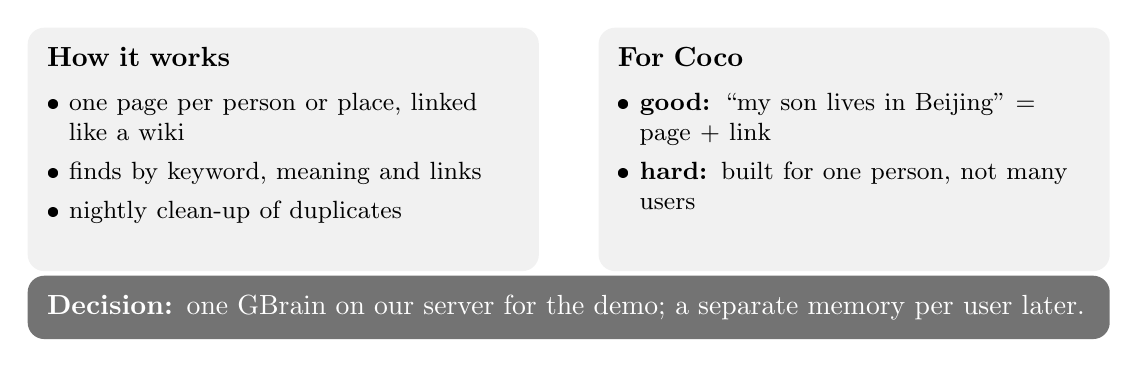
\begin{tikzpicture}
    \node[card,text width=6.0cm] at (0,0) {\topbox{6.0cm}{2.6cm}{%
      \textbf{How it works}\par\vspace{0.5em}\small
      \bul{one page per person or place, linked like a wiki}
      \bul{finds by keyword, meaning and links}
      \bul{nightly clean-up of duplicates}}};
    \node[card,text width=6.0cm] at (7.25,0) {\topbox{6.0cm}{2.6cm}{%
      \textbf{For Coco}\par\vspace{0.5em}\small
      \bul{\textbf{good:} ``my son lives in Beijing'' = page + link}
      \bul{\textbf{hard:} built for one person, not many users}}};
    \node[card,dark,text width=13.25cm] at (0,-3.15) {%
      \textbf{Decision:} one GBrain on our server for the demo; a separate memory per user later.};
  \end{tikzpicture}
\end{frame}

% ───────────────────────── 8. next two weeks ─────────────────────────
\begin{frame}[t]{Next two weeks}
  \vspace*{-0.1cm}
  \begin{columns}[T,onlytextwidth]
    \begin{column}{0.68\textwidth}
      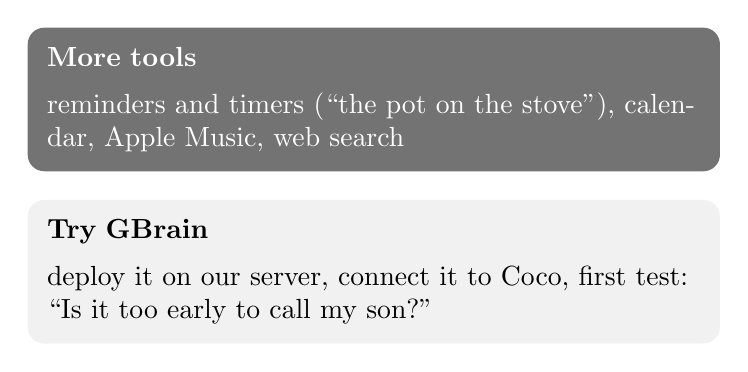
\begin{tikzpicture}
        \node[card,dark,text width=8.3cm] (a) at (0,0) {%
          \textbf{More tools}\\[0.5em]
          reminders and timers (``the pot on the stove''), calendar, Apple Music, web search};
        \node[card,text width=8.3cm,anchor=north west] at ([yshift=-0.35cm]a.south west) {%
          \textbf{Try GBrain}\\[0.5em]
          deploy it on our server, connect it to Coco, first test: ``Is it too early to call my son?''};
      \end{tikzpicture}
    \end{column}
    \begin{column}{0.29\textwidth}
      \centering
      \vspace{0.3cm}
      
\includegraphics[width=\textwidth]{panda-thinking}
    \end{column}
  \end{columns}
  \vfill
  \noindent{\small\color{soft}Code: \href{https://github.com/renxingyu0822-cmd/Coco}{github.com/renxingyu0822-cmd/Coco}}\par\vspace{0.1cm}
\end{frame}

\end{document}
